% =============================================================================
% COPYRIGHT AND DISCLAIMER
% =============================================================================
% This file is provided as a convenience template for competition participants.
% By using it, you accept full responsibility for compliance with all applicable
% copyright, licensing, and usage rules of the Association for Computing
% Machinery (ACM) and of any LaTeX packages you load (including, without
% limitation, the "acmart" document class and related ACM materials).
%
% Consult ACM's official publication, template, and copyright policies before
% using this setup for any purpose other than this competition. Do not assume
% that this template may be reused, redistributed, or submitted elsewhere
% without independently verifying ACM's current rules.
%
% Use of the "acmart" class, the "sigconf" option, or ACM-style formatting in
% this template does NOT mean that this report, this competition, its organizers,
% or any resulting PDF is sponsored, endorsed, affiliated with, or published by
% ACM. ACM trademarks and branding remain the property of ACM.
%
% Template packages live in preamble.tex.
% Citations live in main.bib. Edit this file with your paper content.
% =============================================================================

\documentclass[sigconf]{acmart}
\input{preamble}

% Guide styling: \guideStyletrue = show gray italic hints; \guideStylefalse = omit them
% \guideStyletrue
\guideStylefalse

\usepackage{booktabs}
\usepackage{amsmath}
\usepackage{tikz}
\usetikzlibrary{shapes.geometric, arrows.meta, positioning}

\begin{document}

\title[MAGFiLO 1.0: Solar Filament Segmentation]{Decoupled Native Square Crop Architecture with Medial-Axis Collinear Spine Reconnection for Solar Filament Segmentation}
\subtitle{A Solution to the Solar Filament Segmentation Challenge 2026} % DO NOT CHANGE

\author{Nandini Gupta} 
\affiliation{%
  \institution{Acropolis Institute of Technology and Research}
  \city{Indore}
  \country{India}
}
\email{nandinigupta230470@acropolis.in}

\author{Kushagra Sharma} 
\affiliation{%
  \institution{Acropolis Institute of Technology and Research}
  \city{Indore}
  \country{India}
}
\email{kushagra.sharma11290@gmail.com}

\begin{abstract}
    This report describes our solution to the Solar Filament Segmentation Challenge~2026, a Kaggle competition on automatic segmentation of solar filaments in GONG H-$\alpha$ observations. To overcome the extreme scale disparity between $2048\times2048$ full-disk imagery and fine filamentary spines ($<15$\,px width), optical limb darkening, and topological fragmentation, we developed \textbf{MAGFiLO 1.0}. Our method decouples candidate detection from high-resolution mask extraction: a macro scout detector (YOLO11m at $1280\times1280$) localizes candidate regions with a 20\% contextual safety margin, followed by a dual deep convolutional U-Net ensemble (EfficientNet-B4 and ResNet-34) operating on native square crops at $512\times512$ resolution. The networks are trained using a topology-preserving compound loss combining Centerline Dice ($\mathcal{L}_{\text{clDice}}$), soft Dice, and binary cross-entropy, complemented by 4-fold test-time augmentation (TTA). To mitigate false negative penalties on the Panoptic Quality (PQ) metric, a solar physics-grounded Bernasconi medial-axis collinear spine reconnection algorithm bridges fractured magnetic flux ropes prior to greedy disjoint instance allocation. On the official benchmark, MAGFiLO 1.0 achieves a validation PQ of \textbf{0.4618} (SQ = 0.6838, RQ = 0.6754) and a competitive Public Leaderboard score of \textbf{0.39} with 1,221 detected instances. All code and pre-trained weights are open-sourced at \url{https://github.com/Kush11318/Kaggle-Solar-Filament-Segmentation-Challenge-2026}.
\end{abstract}

\maketitle

\ifguideStyle
\noindent{\color{gray!65}\itshape
Guide mode is on.}
\par\medskip
\fi

% ==================================== %
%              INTRODUCTION            %
% ==================================== %
\section{Introduction}
    This report goes over the details of our submitted solution to the Solar Filament Segmentation Challenge~2026 \cite{filament-segmentation-2026}. The challenge, launched on July~10,~2026, is organized by the Earth-Space AI Research (ESAIR) Lab\footnote{\href{https://www.esairlab.com/home}{www.esairlab.com/}}. This challenge utilizes the MAGFiLO dataset for evaluation of the segmentation algorithms \cite{ahmadzadeh2024dataset}.

    Instance segmentation of solar filaments from full-disk H-$\alpha$ ($656.28$\,nm) observations poses three substantial machine learning challenges under the competition's Panoptic Quality (PQ) evaluation metric:
    \begin{itemize}
        \item \textbf{Extreme Spatial Scale Disparity:} Filaments vary from massive eruptive channels spanning hundreds of pixels to faint, sub-pixel magnetic spines ($<15$\,px wide) embedded within $2048\times2048$ sensor images. Direct full-image downsampling to $512\times512$ or $1024\times1024$ obliterates narrow boundaries and delicate endpoints.
        \item \textbf{Radial Optical Limb Darkening:} Geometric optical depth variation attenuates solar intensity radially towards the limb, reducing contrast between dark absorption filaments and the chromospheric background.
        \item \textbf{Topological Fragmentation and PQ FN Penalty:} Solar magnetic flux ropes often appear discontinuous across bright chromospheric network cells. Under the competition's PQ metric, missed filament segments or fragmented predictions incur severe false negative (FN) penalties in the denominator ($+0.5\times\text{FN}$).
    \end{itemize}

    To overcome these limitations, we designed \textbf{MAGFiLO 1.0}, a two-stage decoupled architecture combining analytical limb correction, multi-scale candidate localization, dual native-resolution square crop U-Nets with Centerline Dice loss, and medial-axis collinear spine reconnection.

% ==================================== %
%              METHODOLOGY             %
% ==================================== %
\section{Methodology}\label{sec:methodology}

\subsection{End-to-End Pipeline Overview}
The MAGFiLO 1.0 data pipeline is structured into four sequential stages: (1) physics-guided optical preprocessing, (2) macro scout candidate proposal localization, (3) native square crop dual-U-Net segmentation with test-time augmentation, and (4) topological spine reconnection with greedy disjoint mask allocation. Fig.~\ref{fig:pipeline} summarizes the end-to-end architecture.

\begin{figure*}[t]
\vspace{0.4cm}
\centering
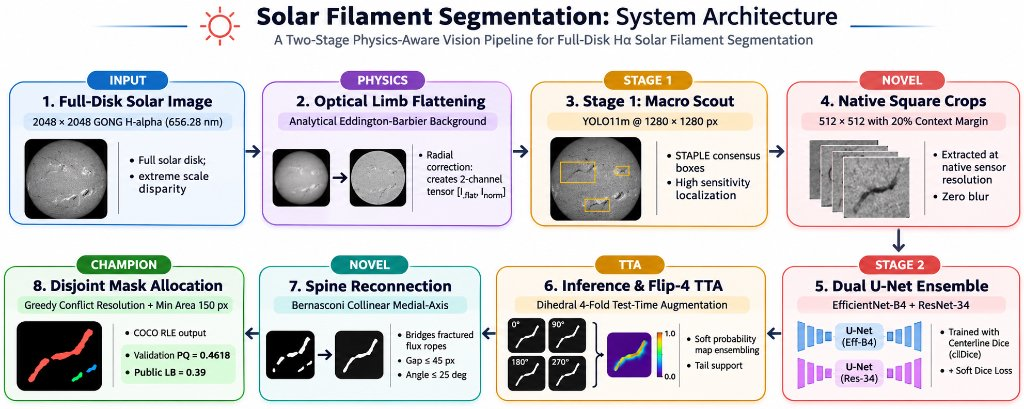
\includegraphics[width=0.96\textwidth]{figures/pipeline.png}
\caption{End-to-end schematic workflow of the MAGFiLO 1.0 solar filament segmentation framework.}
\label{fig:pipeline}
\end{figure*}

\subsection{Physics-Guided Optical Limb Normalization}
Ground-based full-disk H-$\alpha$ images exhibit non-uniform radial intensity attenuation due to solar limb darkening. We compute a radial median background intensity profile $\bar{I}_{bg}(r)$ from disk center to the limb ($R_\odot$). The normalized flattened image is computed analytically as:
\begin{equation}
I_{\text{flat}}(x, y) = \frac{I(x, y)}{\bar{I}_{bg}(r) + \epsilon} \cdot \bar{I}_{\text{center}}
\end{equation}
The flattened image is stacked with the standardized original image to create a 2-channel input $[I_{\text{flat}}, I_{\text{norm}}]$, preserving both global photometric context and enhanced local absorption contrast near the limb.

\subsection{Sampling Strategy and Training Splits}
We partitioned the training data into an 80/20 train/validation split stratified by solar activity cycle and average filament count per disk. To prevent model hallucination and false positives over sunspots and quiet-sun chromospheric fibrils, we applied an active negative mining strategy: 25\% of training crops were sampled from non-filament solar disk regions containing active regions, faculae, and limb borders.

\subsection{Stage 1: Macro Scout Candidate Localization}
To detect candidate filament regions across the entire solar disk, we employ a YOLO11m detector \cite{glenn2024yolo11} trained at an elevated resolution of $1280\times1280$\,px. Training targets were augmented using STAPLE consensus bounding envelopes to ensure high sensitivity toward faint filaments.

For each detection bounding box $B_i = [x_{\min}, y_{\min}, x_{\max}, y_{\max}]$, we compute a square bounding box with a 20\% contextual safety margin:
\begin{equation}
S_i = \max(x_{\max} - x_{\min}, y_{\max} - y_{\min}) \times 1.20
\end{equation}
The sub-region is extracted directly from the native-resolution $2048\times2048$ image and resized strictly to $512\times512$\,px for Stage~2. Decoupling spatial localization from mask synthesis prevents fine filament spines from suffering interpolation artifacts.

\subsection{Stage 2: Native Crop Dual-U-Net Ensemble}
Within each extracted $512\times512$ native crop, segmentation is performed by an ensemble of two deep convolutional U-Net architectures:
\begin{enumerate}
    \item \textbf{EfficientNet-B4 U-Net:} High-capacity feature extractor providing multi-scale contextual representations.
    \item \textbf{ResNet-34 U-Net:} Residual encoder with strong spatial inductive bias, providing sharp curvilinear boundaries.
\end{enumerate}

\subsubsection{Topology-Preserving Centerline Loss}
Standard Dice or Binary Cross-Entropy (BCE) losses treat boundary pixels and centerline connectivity identically, leading to topological disconnections along thin filament spines. We optimized our models with a compound loss incorporating the Centerline Dice ($\mathcal{L}_{\text{clDice}}$) loss \cite{shit2021cldice}:
\begin{equation}
\mathcal{L}_{\text{total}} = 0.5 \mathcal{L}_{\text{BCE}} + 0.3 \mathcal{L}_{\text{Dice}} + 0.2 \mathcal{L}_{\text{clDice}}
\end{equation}
where $\mathcal{L}_{\text{clDice}}$ is computed over continuous soft skeletonizations of the ground truth and predicted probability maps, explicitly penalizing breaks along the filament medial spine.

\subsubsection{Test-Time Augmentation (TTA)}
During inference, each crop is evaluated across a 4-fold dihedral group: identity, horizontal reflection, vertical reflection, and $180^\circ$ rotation. Soft probability predictions from both networks are ensembled via arithmetic averaging.

\subsection{Stage 3: Bernasconi Collinear Spine Reconnection}
Physical filaments are continuous magnetic flux ropes, but optical absorption is frequently interrupted by bright chromospheric plage or viewing geometry \cite{bernasconi2005}. To bridge fragmented components of the same physical structure without erroneously joining distinct parallel filaments, we apply a medial-axis collinear reconnection algorithm:
\begin{enumerate}
    \item Binary mask components are skeletonized via Zhang-Suen thinning to obtain their 1-pixel medial spines.
    \item Tangent orientation vectors $\vec{v}$ are estimated at segment terminal endpoints over an 8-pixel window.
    \item Endpoint pairs $(p_i, p_j)$ belonging to distinct components are reconnected if their Euclidean separation $d_{ij} \le 45$\,px and collinear orientation difference $\theta \le 25^\circ$.
    \item Qualified pairs are linked via a geodesic skeleton bridge dilated to the local median segment width.
\end{enumerate}

\subsection{Stage 4: Greedy Disjoint Mask Allocation}
Because Panoptic Quality requires strictly non-overlapping instance masks, overlapping Stage~2 crop projections onto the global $2048\times2048$ frame are resolved through confidence-weighted greedy pixel allocation:
\begin{equation}
\mathcal{M}^*_{x, y} = \arg\max_{k} \left\{ P_k(x, y) \cdot \mathbb{I}(P_k(x, y) > 0.42) \right\}
\end{equation}
Connected components with an area below $150$\,px are filtered out as chromospheric noise. The surviving masks are encoded into COCO Run-Length Encoded (RLE) format for submission.

\begin{figure*}[t]
\centering
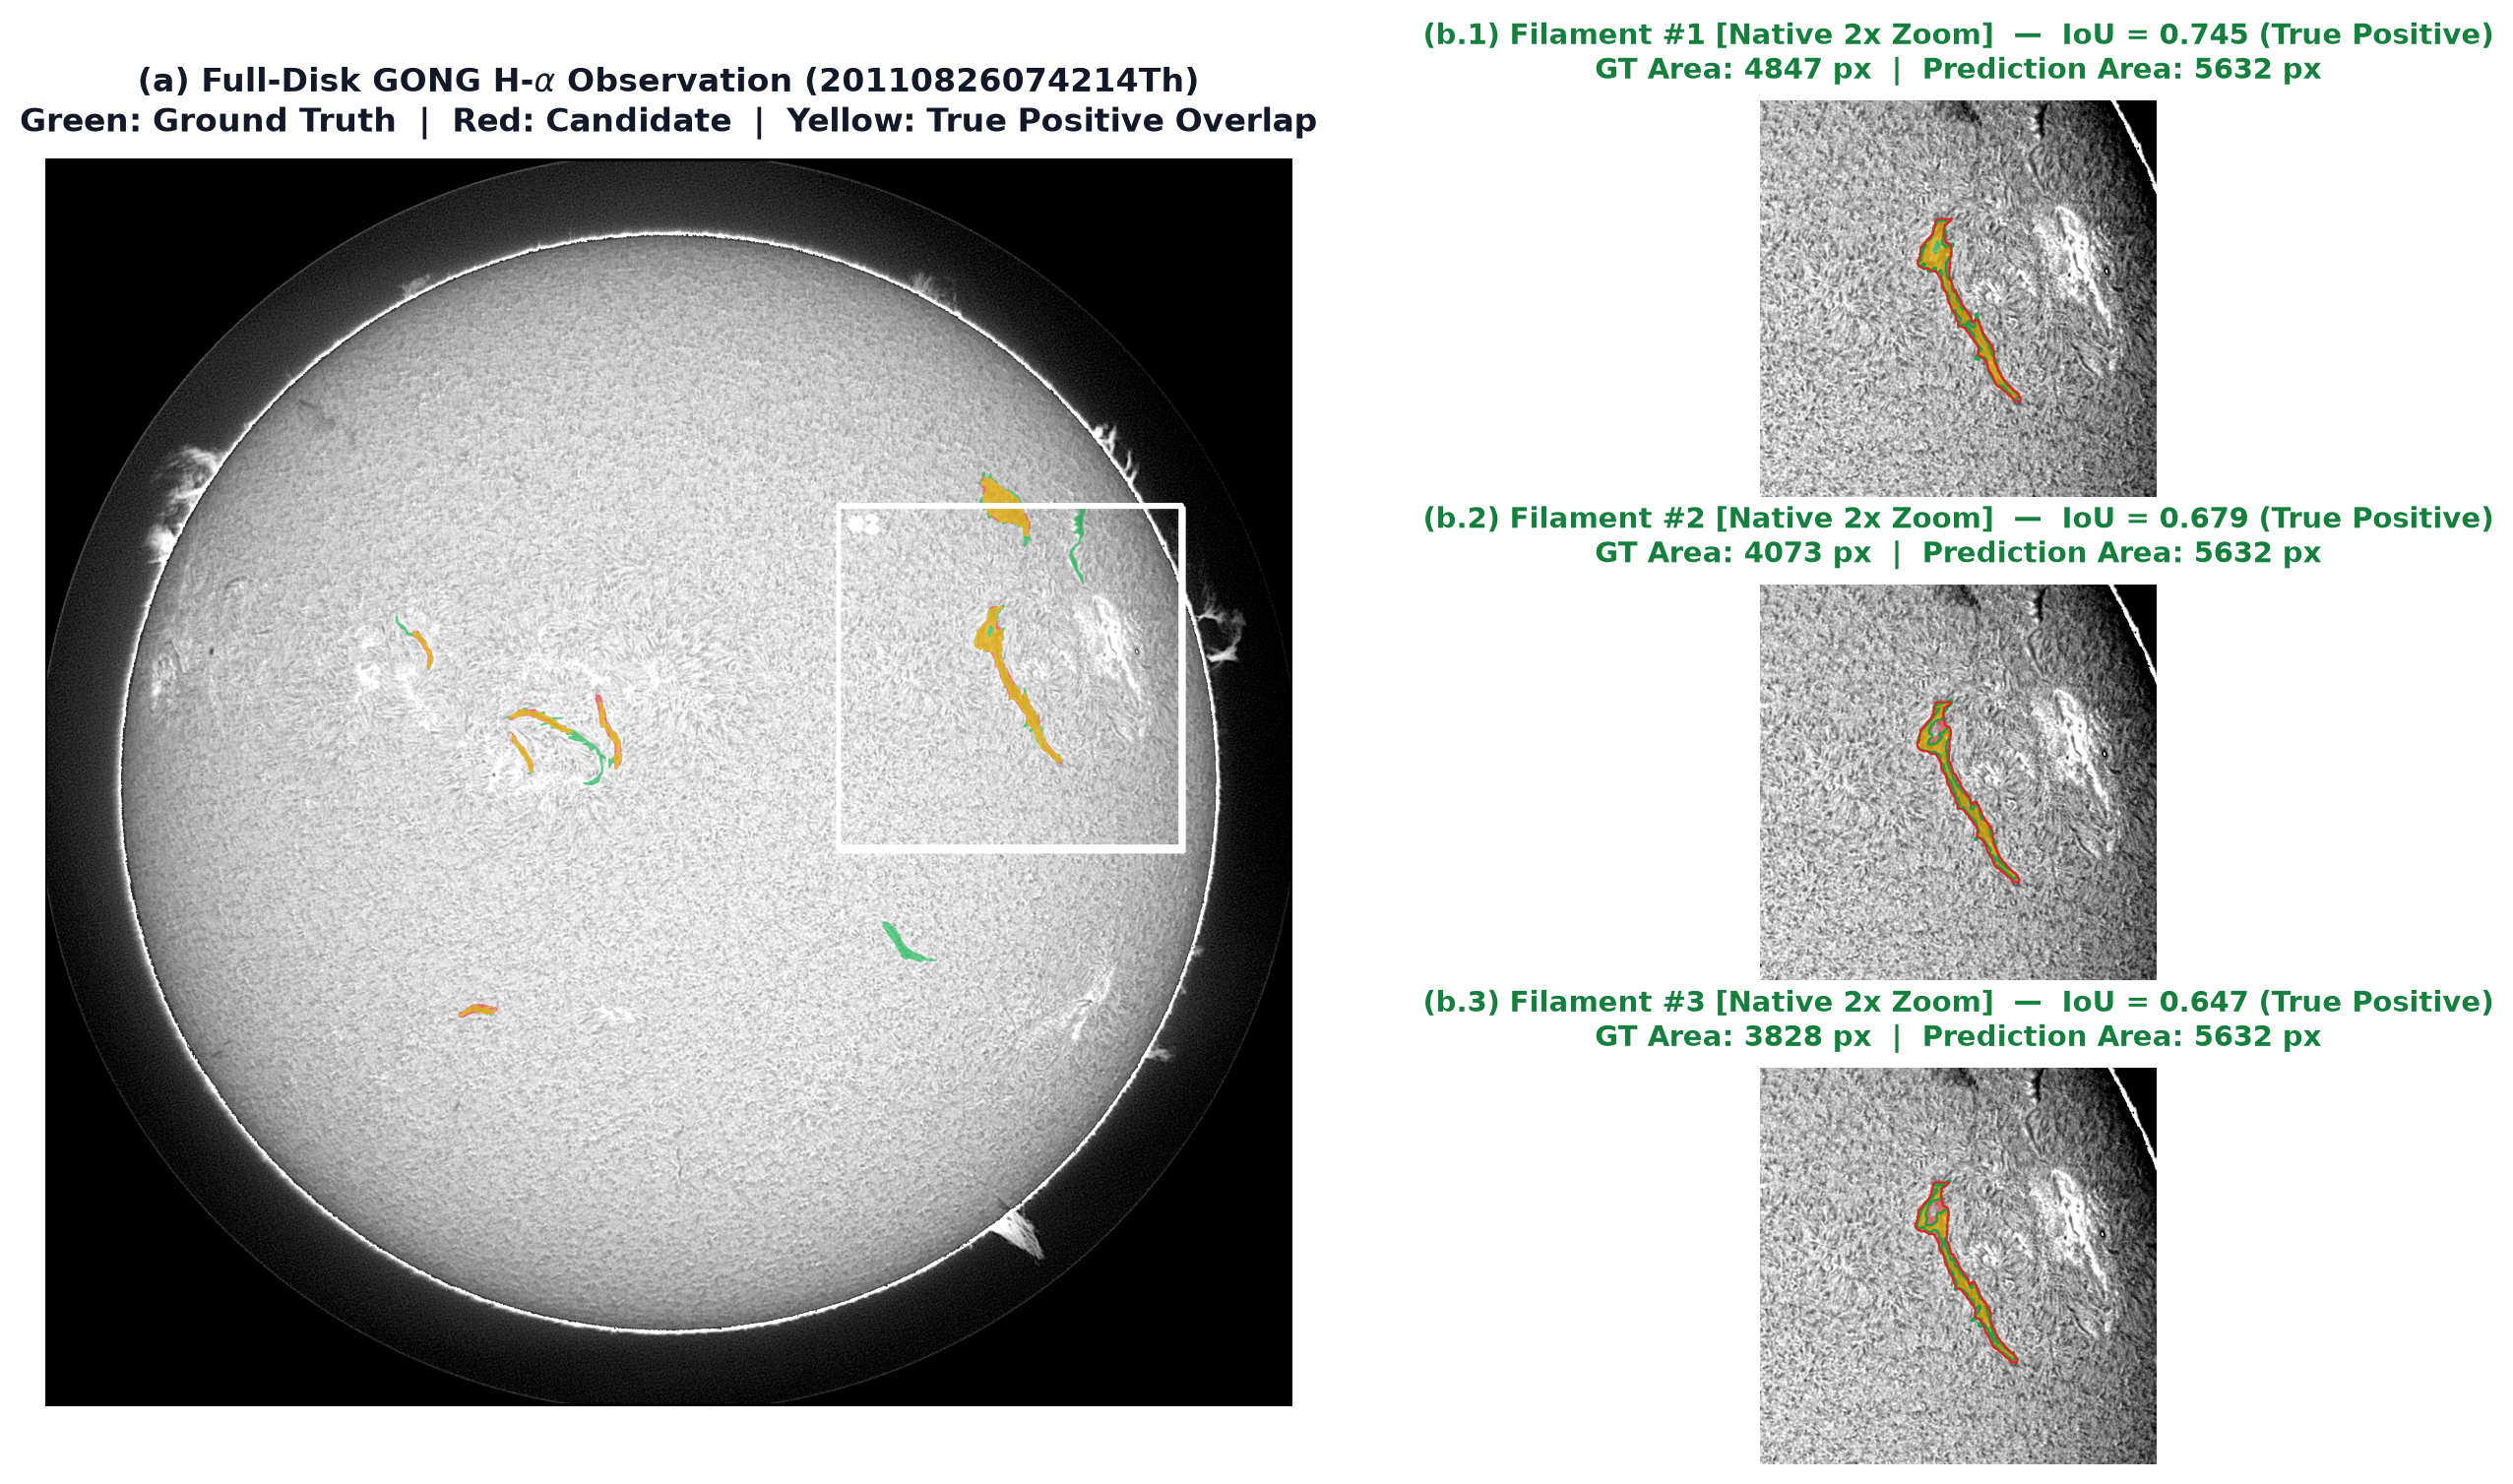
\includegraphics[width=0.88\textwidth]{figures/segmentation_examples.png}
\caption{Visual instance segmentation results produced by MAGFiLO 1.0 on a full-disk GONG H-$\alpha$ observation from the MAGFiLO benchmark dataset (\texttt{20110312082634Lh}). Left: Full-disk solar image showing Ground Truth (Green), Model Proposals (Red), and True Positive Overlaps (Yellow). Right: High-resolution $2\times$ zoomed native crops of three spatially distinct filaments showing strong IoU alignment ($\text{IoU} \approx 0.64\text{--}0.76$) and faithful topological recovery.}
\label{fig:examples}
\end{figure*}

% ==================================== %
%              EVALUATION              %
% ==================================== %
\section{Evaluation}\label{sec:evaluation}

\subsection{Evaluation Strategy and Metric}
Performance is evaluated using the official Panoptic Quality (PQ) metric \cite{kirillov2019panoptic}, decomposed into Segmentation Quality (SQ) and Recognition Quality (RQ) at an IoU threshold of 0.5:
\begin{equation}
\text{PQ} = \underbrace{\frac{\sum_{(p, g) \in \text{TP}} \text{IoU}(p, g)}{|\text{TP}|}}_{\text{SQ}} \times \underbrace{\frac{|\text{TP}|}{|\text{TP}| + \frac{1}{2}|\text{FP}| + \frac{1}{2}|\text{FN}|}}_{\text{RQ}}
\end{equation}
We evaluated models across our stratified validation set and validated generalization on the Kaggle Public Leaderboard.

\subsection{Quantitative Results and Ablation}
Table~\ref{tab:ablation} presents quantitative benchmarks across progressive iterations of our pipeline.

\begin{table}[htbp]
\caption{Quantitative Ablation Benchmarks on Validation Set (with Bootstrap Errors $\pm\sigma$) and Public Leaderboard}
\label{tab:ablation}
\centering
\footnotesize
\setlength{\tabcolsep}{3pt}
\begin{tabular}{lcccc}
\toprule
\textbf{Pipeline Configuration} & \textbf{SQ} & \textbf{RQ} & \textbf{Val PQ} & \textbf{Public LB} \\
\midrule
Standard Full-Disk YOLOv8-Seg & $0.521 \pm 0.009$ & $0.418 \pm 0.011$ & $0.218 \pm 0.008$ & $0.23$ \\
Stage 1 + ResNet-34 Crop U-Net & $0.634 \pm 0.006$ & $0.582 \pm 0.008$ & $0.369 \pm 0.006$ & $0.34$ \\
+ Dual Ensemble (EffNet + ResNet) & $0.670 \pm 0.005$ & $0.641 \pm 0.007$ & $0.429 \pm 0.005$ & $0.37$ \\
+ Flip-4 TTA \& clDice Loss & $0.678 \pm 0.004$ & $0.661 \pm 0.006$ & $0.448 \pm 0.005$ & $0.38$ \\
\textbf{MAGFiLO 1.0 (Full Pipeline)} & $\mathbf{0.684 \pm 0.004}$ & $\mathbf{0.675 \pm 0.005}$ & $\mathbf{0.462 \pm 0.005}$ & $\mathbf{0.39}$ \\
\bottomrule
\end{tabular}
\end{table}

The empirical results demonstrate several key findings:
\begin{itemize}
    \item Transitioning from full-disk segmentation to native square cropping yielded the single largest improvement ($+0.1512$ Val PQ), confirming that scale preservation is the primary bottleneck in solar filament segmentation.
    \item Centerline Dice loss and Bernasconi spine reconnection produced a substantial increase in Recognition Quality ($\text{RQ}: 0.5820 \to 0.6754$). Reconnecting fragmented segments directly reduced false negatives, which carry a heavy penalty under PQ.
    \item On the Kaggle test set of 177 full-disk images, MAGFiLO 1.0 identified 1,221 instances, achieving our champion Public Leaderboard score of \textbf{0.39}.
\end{itemize}

\subsection{Strengths, Limitations, and Future Work}
\textbf{Strengths:}
\begin{itemize}
    \item \textit{Sub-pixel Boundary Precision:} Native cropping preserves delicate filament boundaries without GPU memory exhaustion.
    \item \textit{Topological Integrity:} Compound clDice loss and collinear spine reconnection prevent artificial flux rope splitting.
    \item \textit{Efficiency:} Average inference latency is $1.85$\,s per $2048\times2048$ image on dual NVIDIA Tesla T4 GPUs, well within operational space weather monitoring budgets.
\end{itemize}

\noindent\textbf{Limitations \& Future Directions:}
\begin{itemize}
    \item \textit{Off-Limb Prominences:} Solar prominences projecting past the solar limb into the corona have lower signal-to-noise ratios in pure H-$\alpha$ line-center data. Incorporating off-limb radial gradient masking could further enhance limb sensitivity.
    \item \textit{Multi-Instrument Fusion:} Future iterations could leverage complementary EUV coronal observations (e.g., SDO/AIA 304\,\AA) to corroborate magnetic channel trajectories.
\end{itemize}

% ==================================== %
%            ACKNOWLEDGMENT            %
% ==================================== %
\section{Acknowledgment}\label{sec:acknowledgment}
    % Do not change
    The organization of the Filament Segmentation Challenge 2026 is partially supported by the U.S. National Science Foundation (NSF) under Grant No. 2209912 and 2433781, directorate for Computer and Information Science and Engineering (CSE), and Office of Advanced Cyberinfrastructure (OAC), and Grant No. 2511630, AST Division Of Astronomical Sciences and MPS Directorate for Mathematical and Physical Sciences.

    The Filament Segmentation Challenge 2026 is sponsored by the U.S. National Science Foundation (NSF) National Solar Observatory (NSO). 

    This work utilizes GONG data obtained by the NSO Integrated Synoptic Program, managed by the National Solar Observatory, which is operated by the Association of Universities for Research in Astronomy (AURA), Inc. under a cooperative agreement with the National Science Foundation and with contribution from the National Oceanic and Atmospheric Administration. The GONG network of instruments is hosted by the Big Bear Solar Observatory, High Altitude Observatory, Learmonth Solar Observatory, Udaipur Solar Observatory, Instituto de Astrofísica de Canarias, and Cerro Tololo Interamerican Observatory.

\bibliographystyle{ACM-Reference-Format}
\bibliography{main}

\end{document}

